\chapter{Experiments and Results}

This chapter discusses our experiments that evaluate the performance of the methods described above.

\section{Results}
\todo[inline]{Demonstration of the implementation}

\section{Data}

To evaluate the implementation, we require a set of graphs which will be provided as input to the algorithm. To acquire them, we used the online database The House of Graphs~\cite{HoG} that contains interesting graphs. We decided to conduct experiments on these graphs, as they are most likely to be typical targets of the algorithms. In this work, we experimented with a small subset of all those graphs.

The task of recognising outer \(k\)-planar graphs is NP-hard. Consequently, the resources required by all implemented algorithms grow exponentially with the input size. To be able to perform the experiments, we had to limit the size of the graphs. We have done this by picking only ones with at most \(10\) vertices. This constraint leaves plenty of graphs to experiment with while significantly limiting the requirement for resources. Also, as we designed the implementation only for connected graphs, we filtered out ones with multiple components.

This query resulted in \(2007\) different graphs. Among them \(1326\) are biconnected and \(681\) are not.


\section{Experiment setup}

All experiments described below were conducted on a virtual cloud server provided by Amazon Web Services. The hardware available was limited to a single core of an AWS Graviton4 Processor and 2GiB of random access memory. As an operating system, we used Linux.

For each experiment, we chose a set of graphs, a set of methods and a set of configurations. We construct all possible triplets of these parameters. For each one of them, we find the smallest \(k\) for which the given graph is outer \(k\)-planar using the specified method in a given configuration. Apart from recording the \(k\) itself, we also track the time required by the corresponding algorithm, which does not include the time required to start up and parse the graph, as it is part of any algorithm. Unfortunately, some methods require an unreasonable amount of time to calculate the result for some graphs. To mitigate this, we limit the execution time to \(10\) minutes for each triplet, indicating the outcome in the results.

We save the results of each experiment in the \textsc{csv} format. For each entry, we specify the Graphviz representation of the graph, the configuration, the method, and the execution results. The latter includes crossing number \(k\), the time required to find it and whether the algorithm succeeded or not.


\section{Biconnected decomposition}

\begin{figure}[tbh]
    \centering
    \captionsetup{subrefformat=parens}
    \subfloat[ILP]{
        \label{fig:bctree-results:ilp}
        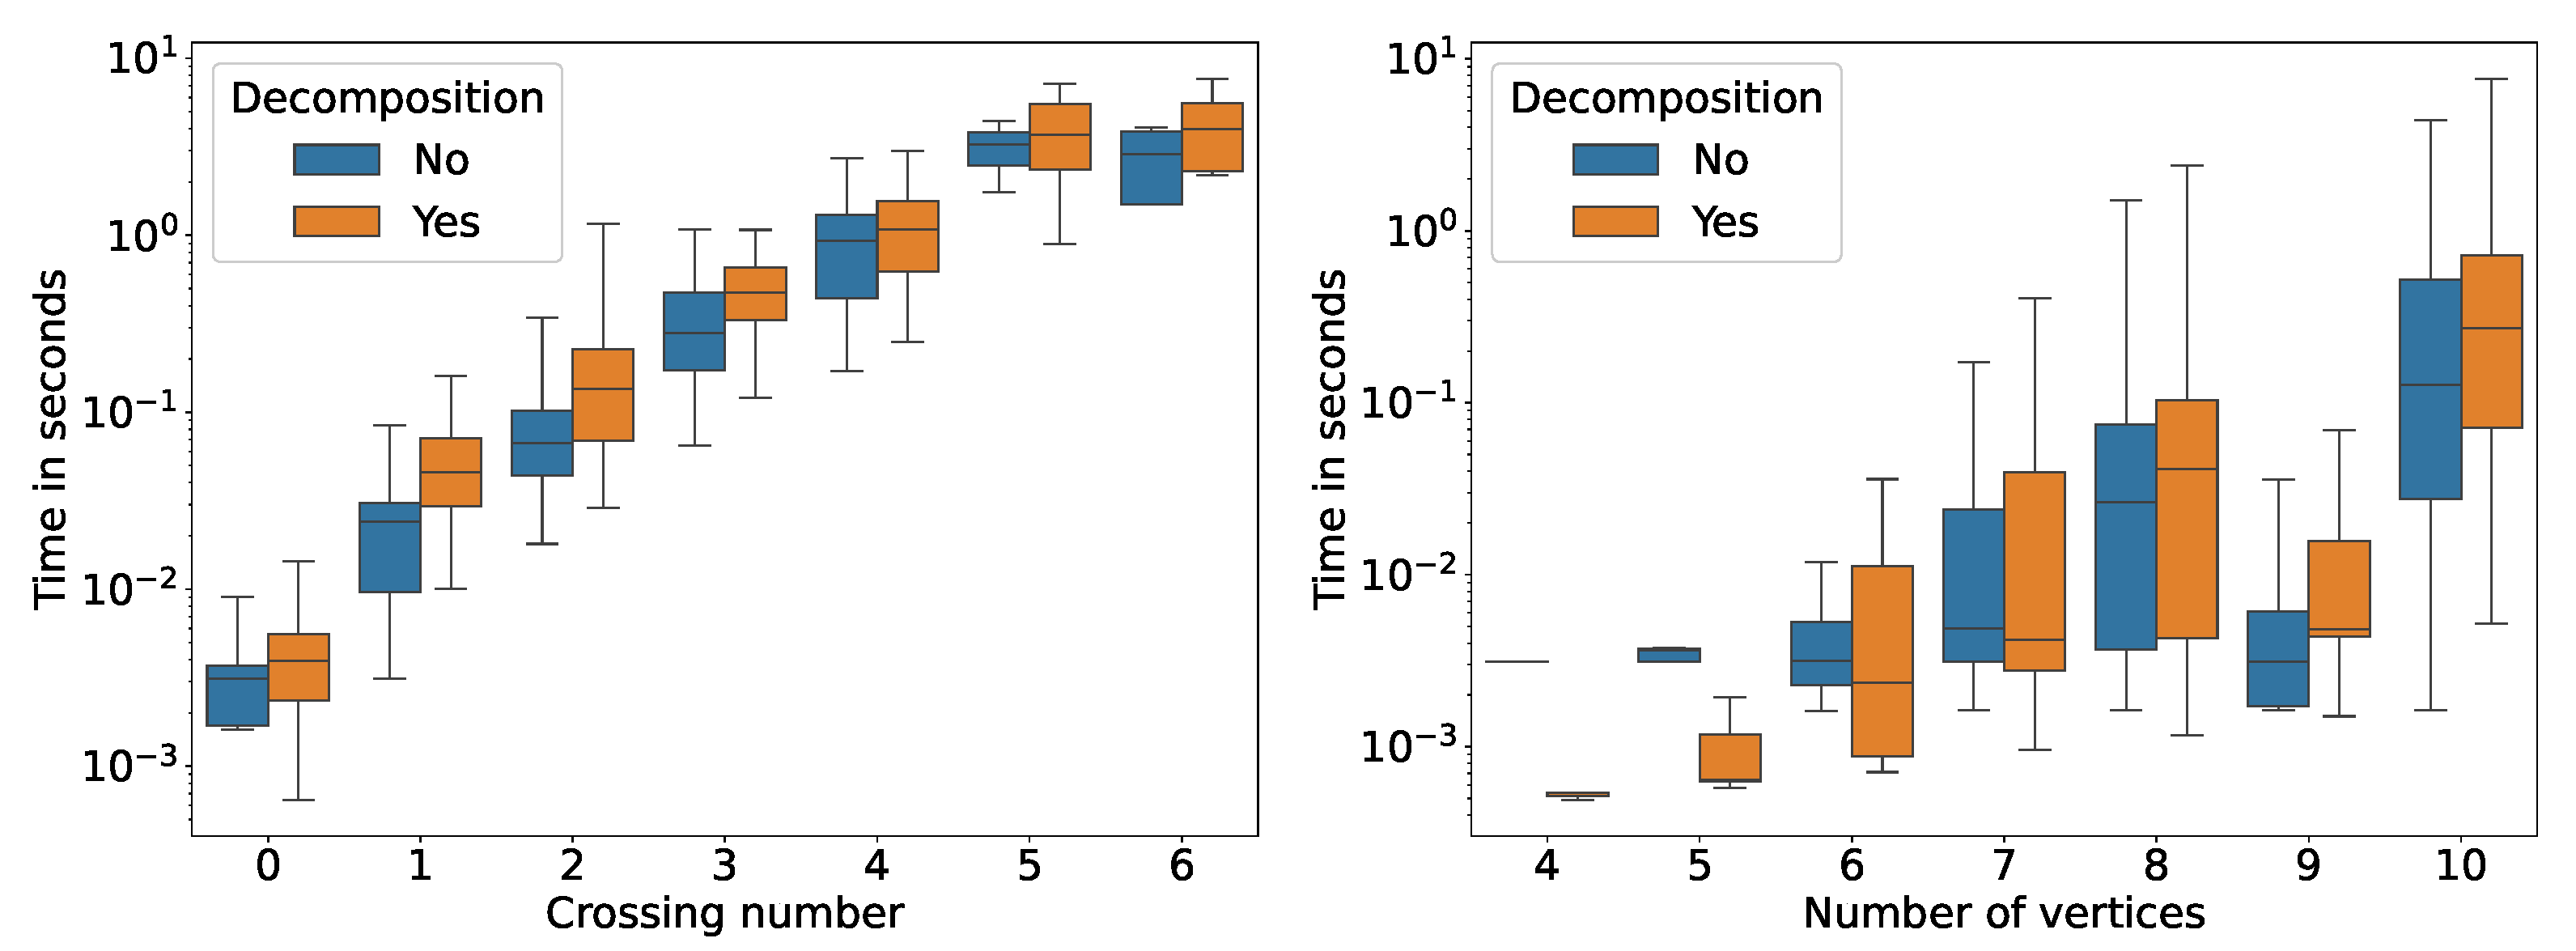
\includegraphics[width=\textwidth]{experiments/bctree_ilp}
    } \hfill
    \subfloat[SAT]{
        \label{fig:bctree-results:sat}
        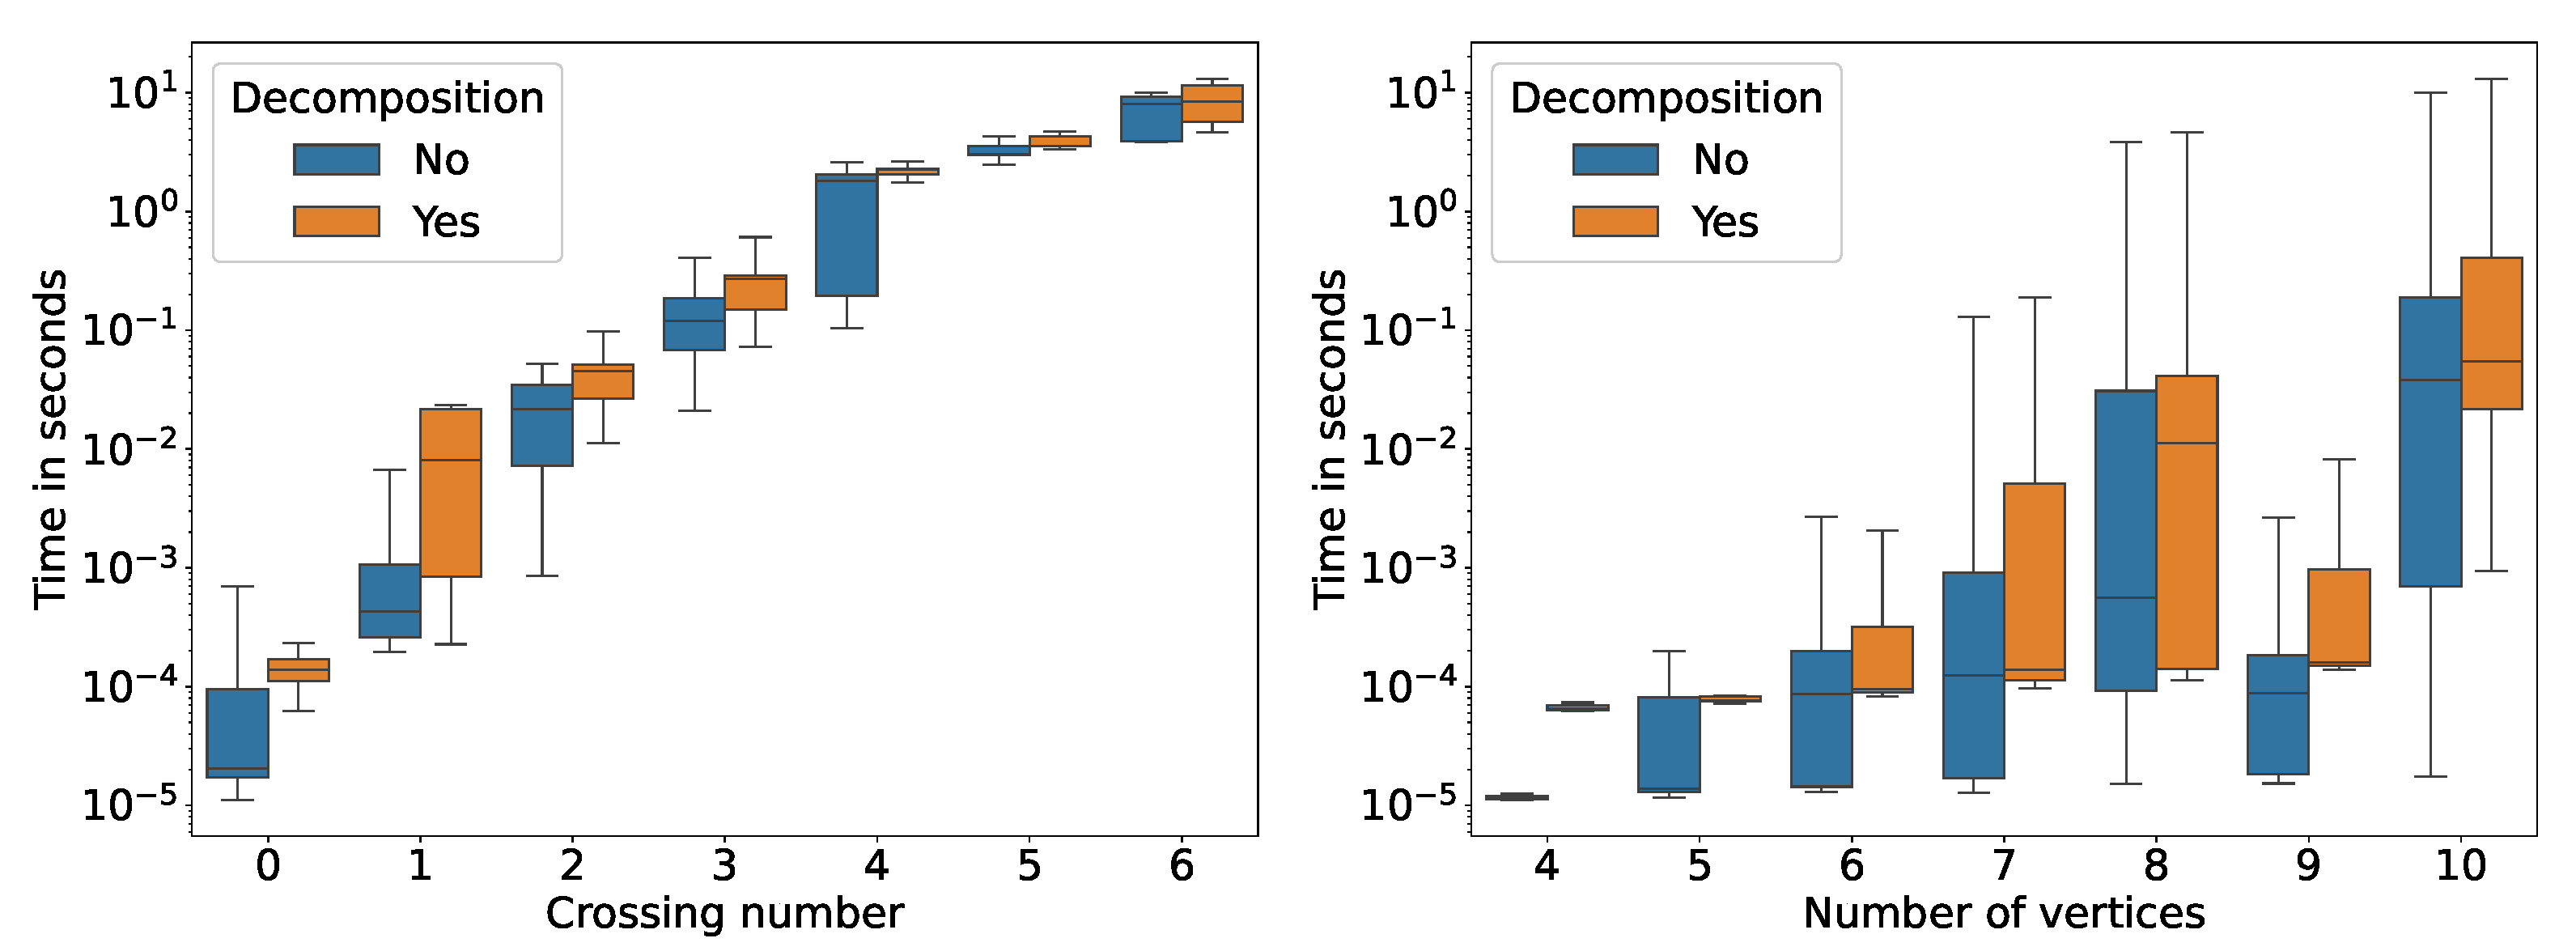
\includegraphics[width=\textwidth]{experiments/bctree_sat}
    } \hfill
    \subfloat[DP]{
        \label{fig:bctree-results:okp}
        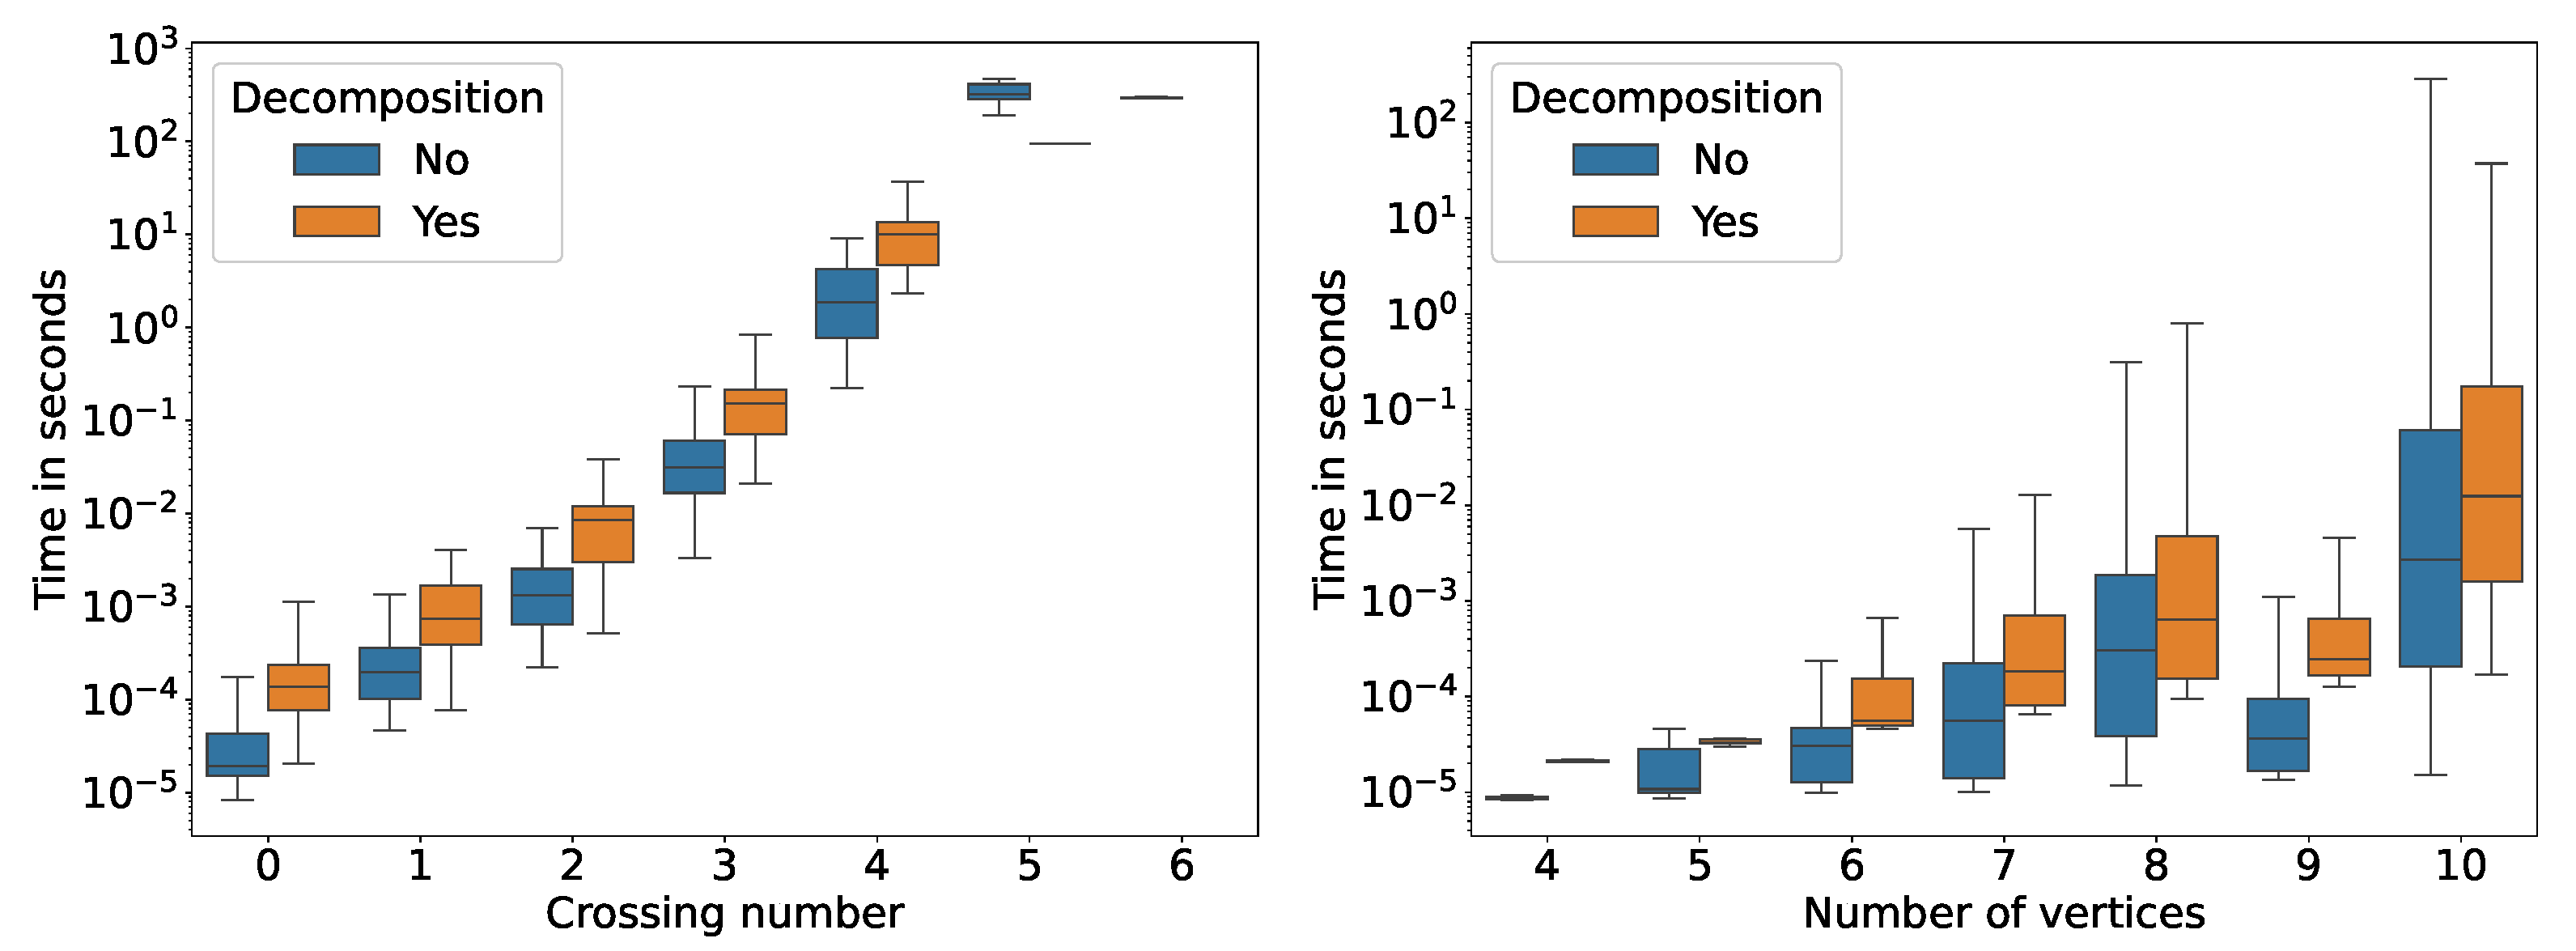
\includegraphics[width=\textwidth]{experiments/bctree_okp}
    }
    \caption{Results of the experiment, demonstrating the influence of biconnected decomposition on the running time of ILP, SAT and DP algorithms.}
    \label{fig:bctree-results}
\end{figure}

The first experiment we considered was comparing the performance of the algorithms with and without bicomponent decomposition. Here, we used only non-biconnected graphs from the dataset to show the difference between the two configurations. We ran this for all three methods. The results are presented in the figure~\ref{fig:bctree-results}.

The results prove that using decomposition indeed boosts performance for almost all methods and graphs. The only exceptions are small graphs for an ILP-based algorithm, for which the cost of initialising multiple environments outweighs the cost of decoupling the problem.

As we demonstrated in this experiment, the non-biconnectivity of the graphs artificially decreases the complexity of the recognition task, as each one of them requires multiple times fewer resources compared to equally sized biconnected graphs. Thus, in the following experiments, we consider only biconnected graphs to exclude this source of noise from the results.


\section{Algorithms conparison}

\begin{figure}[tbh]
    \centering
    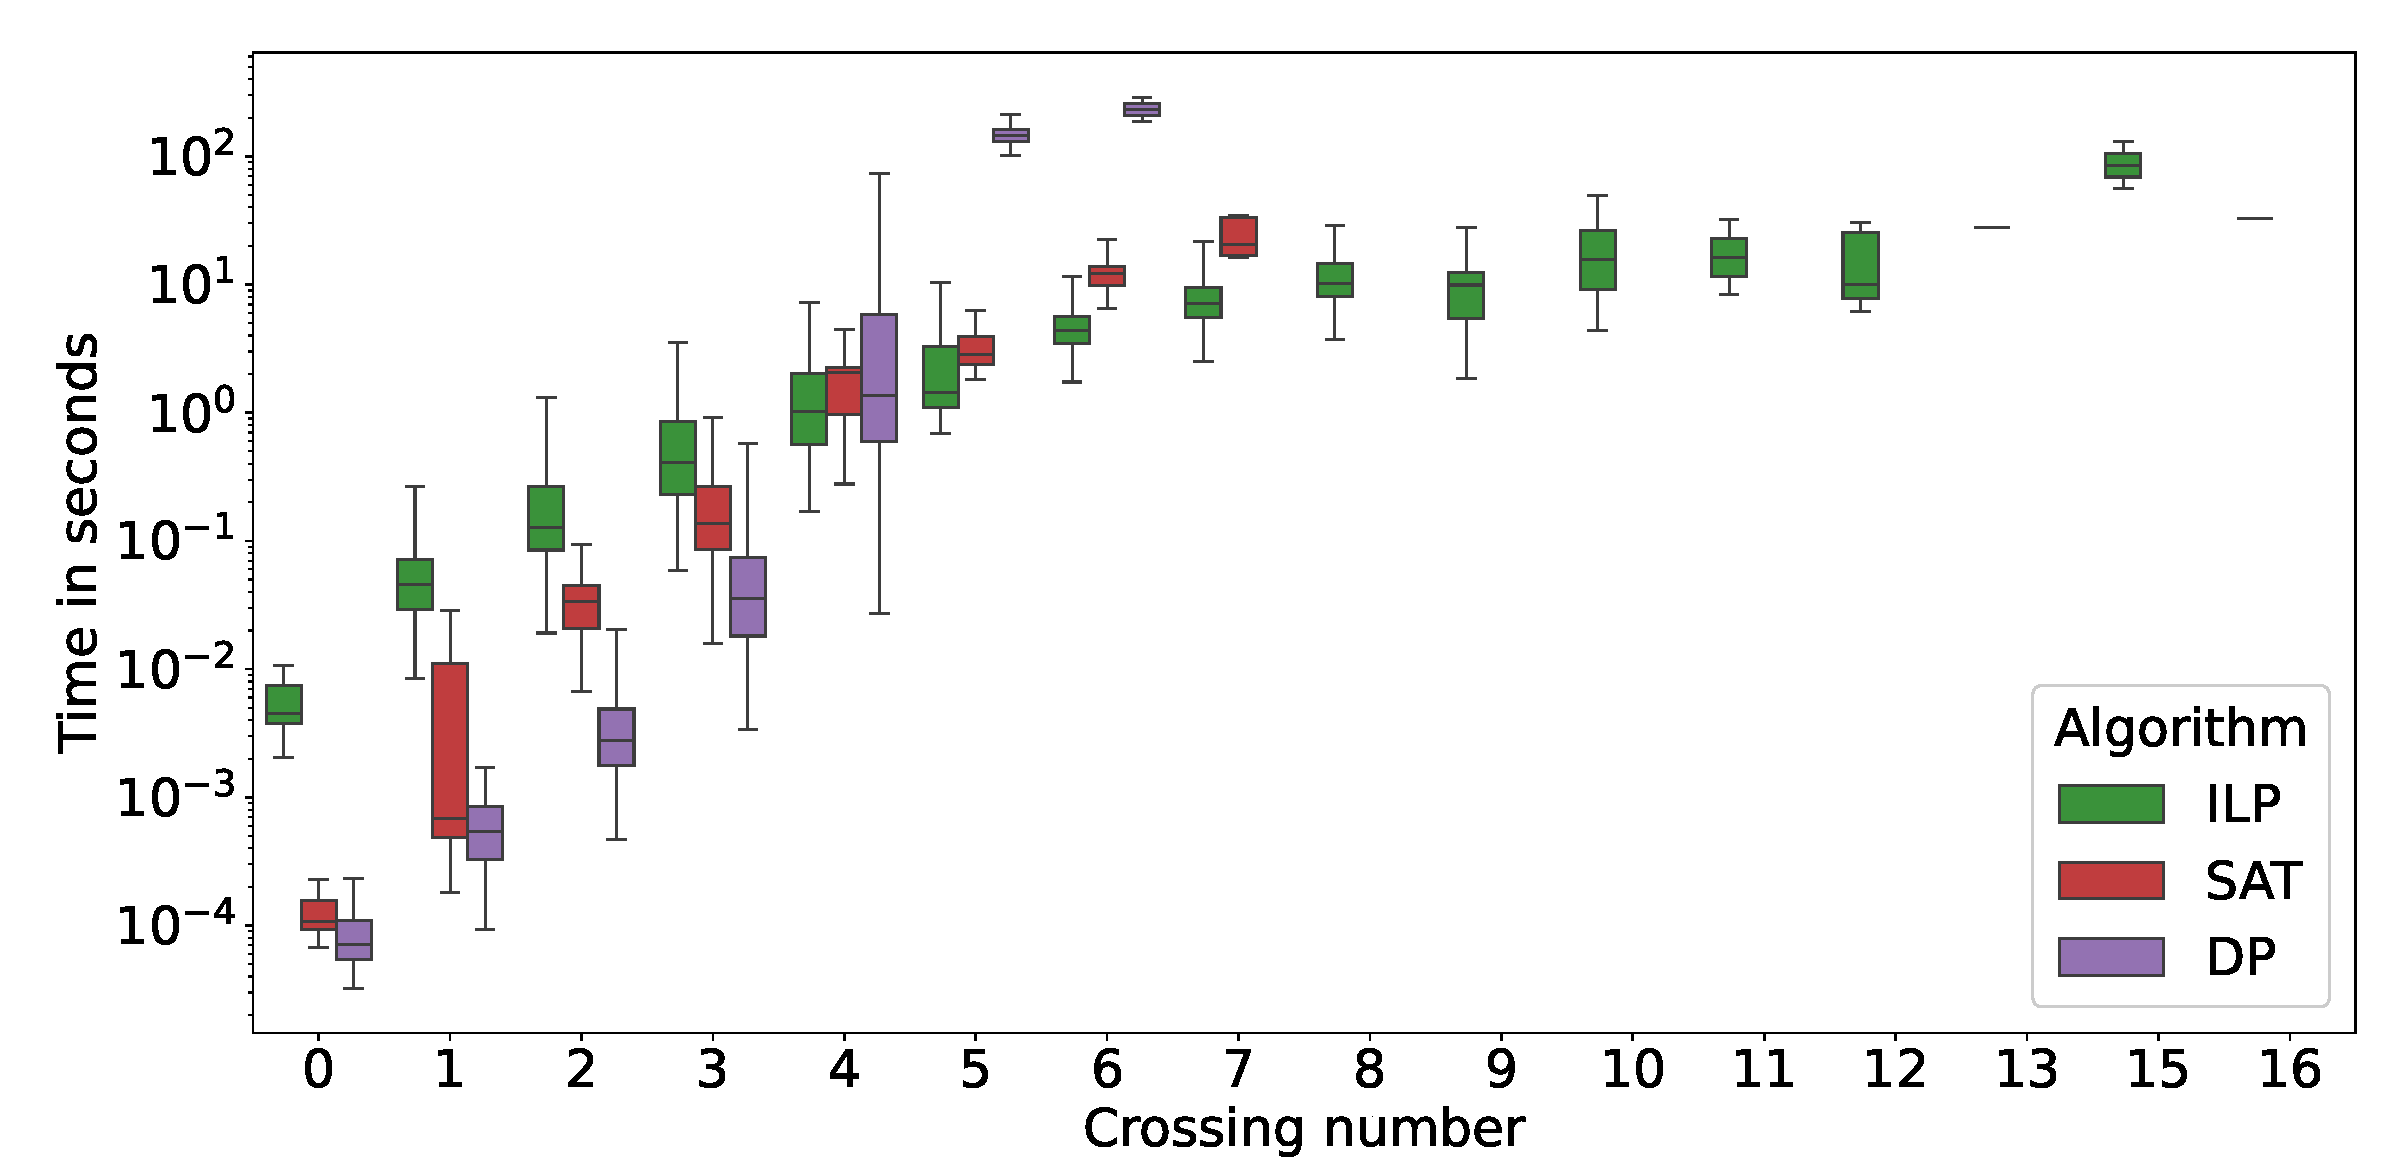
\includegraphics[width=.75\textwidth]{experiments/methods}
    \caption{Comparison of running times of different algorithms for graphs with different crossing numbers.}
    \label{fig:methods}
\end{figure}

In this experiment, we compared the performance of the algorithms. We grouped results by crossing numbers and the algorithm used for solving and displayed in figure~\ref{fig:methods}. Due to the complexity of the problem, some runs ran out of allocated resources. So, to display the results, we used only the measurements from runs that successfully found the minimal crossing number. As a result, starting from \(k = 6\), boxes for SAT and DP algorithms depict fewer runs compared to an ILP algorithm as they required more resources for some graphs than were available.

SAT and DP algorithms, however, were primarily limited by different factors. Unlike ILP, SAT formulation results in a problem that requires an exponential number of clauses to write it down. As a result, the solver ran out of allocated memory for \(185\) out of \(1326\) biconnected graphs. Similarly, the algorithm based on dynamic programming ran out of memory \(16\) times. However, the bigger limiting factor for this algorithm is time, as \(317\) runs exceeded the 10-minute time limit imposed on each one. All other runs finished successfully.

The results show that the time required by both SAT-based and DP algorithms grows much faster than the time required by ILP-based algorithm. The latter requires each instance to set up an environment for the graphs. With smaller crossing numbers, these costs outweigh the solver's speed. However, for instances with bigger \(k\), the time required for setup is negligible.

\begin{figure}[tbh]
    \centering
    \subfloat[\(k = 2\)]{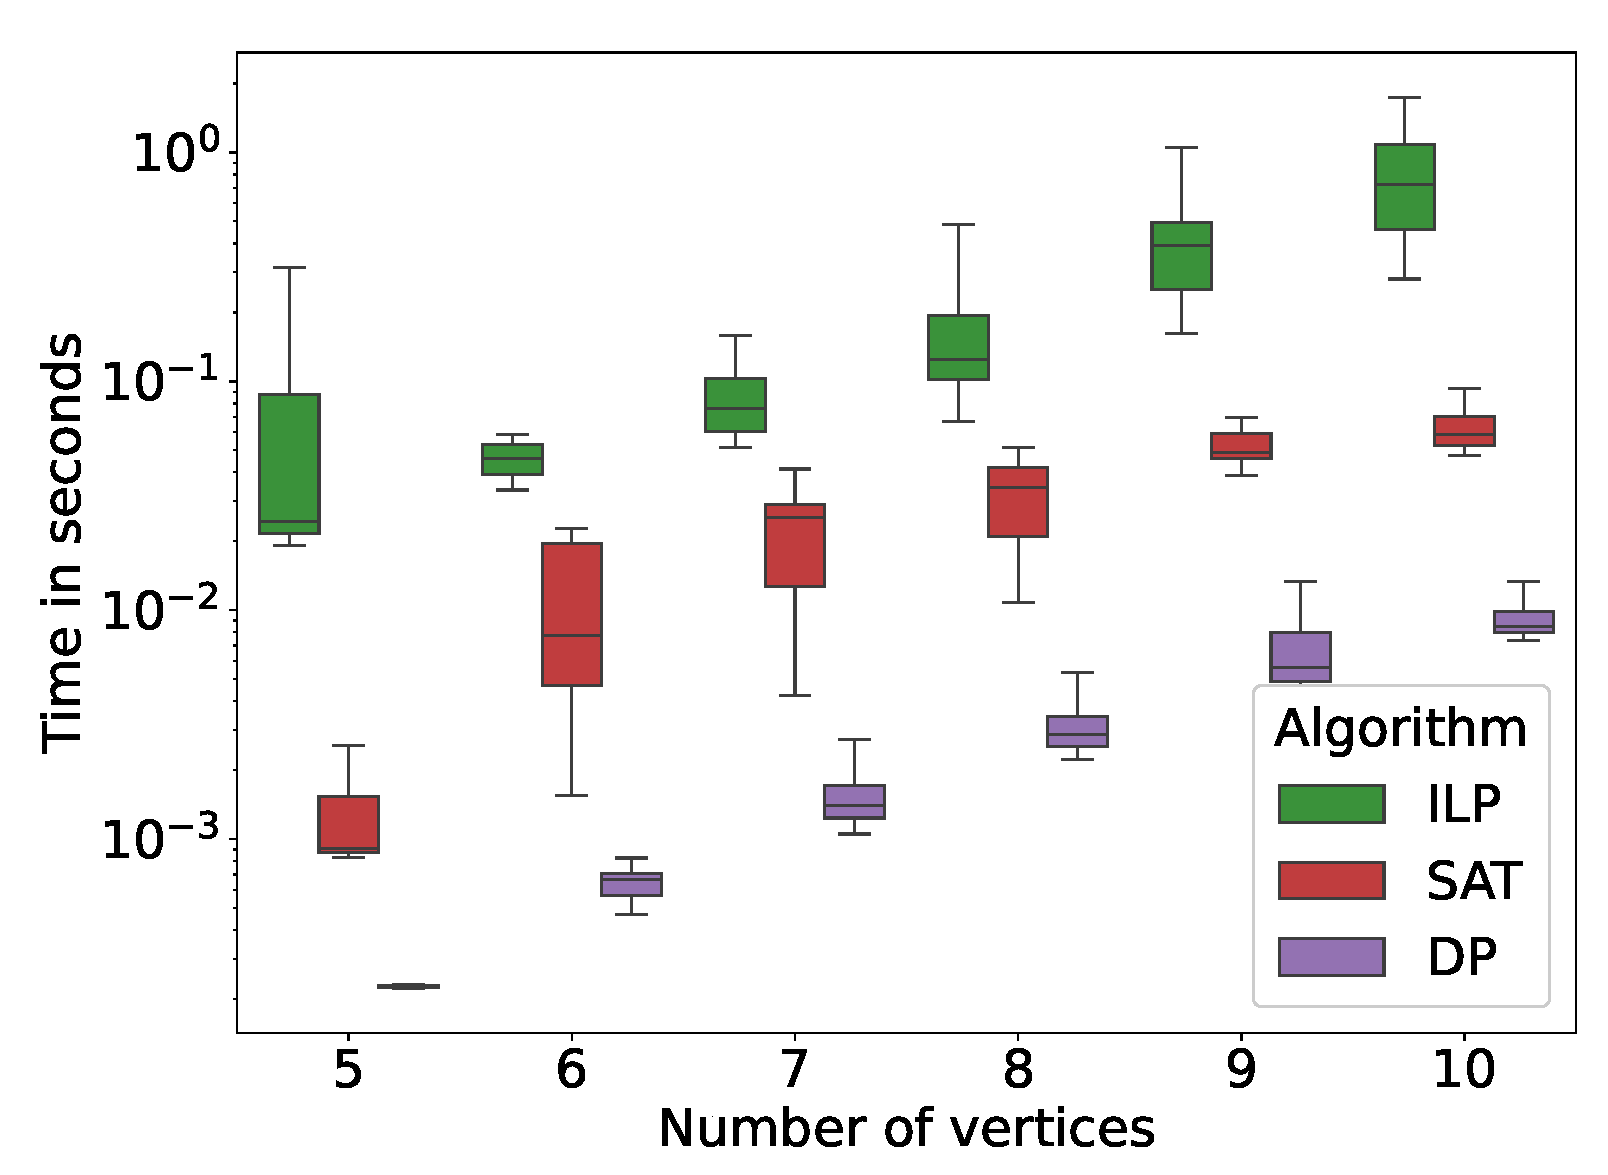
\includegraphics[width=.48\textwidth]{experiments/method_2}} \hfill
    \subfloat[\(k = 3\)]{\includegraphics[width=.48\textwidth]{experiments/method_3}} \hfill
    \subfloat[\(k = 4\)]{\includegraphics[width=.48\textwidth]{experiments/method_4}} \hfill
    \subfloat[\(k = 5\)]{\includegraphics[width=.48\textwidth]{experiments/method_5}} \hfill
    \caption{Comparison of running times required by algorithms to recognise an outer \(k\)-planar graph for different values of \(k\).}
    \label{fig:methods-vertices}
\end{figure}

As the algorithm's running time depends not only on crossing numbers but also on the size of the graph, we can represent the results more accurately by grouping them by both the crossing number and the number of vertices. Such plots for crossing numbers \(2\), \(3\), \(4\) and \(5\) are displayed in figure~\ref{fig:methods-vertices}. In these plots, we can more clearly see the time's dependency on the graph's size.

\todo[inline]{Probably need a little bit more here about figure~\ref{fig:methods-vertices}.}


\section{Optimisation benchmark}

\begin{figure}[tbh]
    \centering
    \subfloat[ILP algorithm]{
        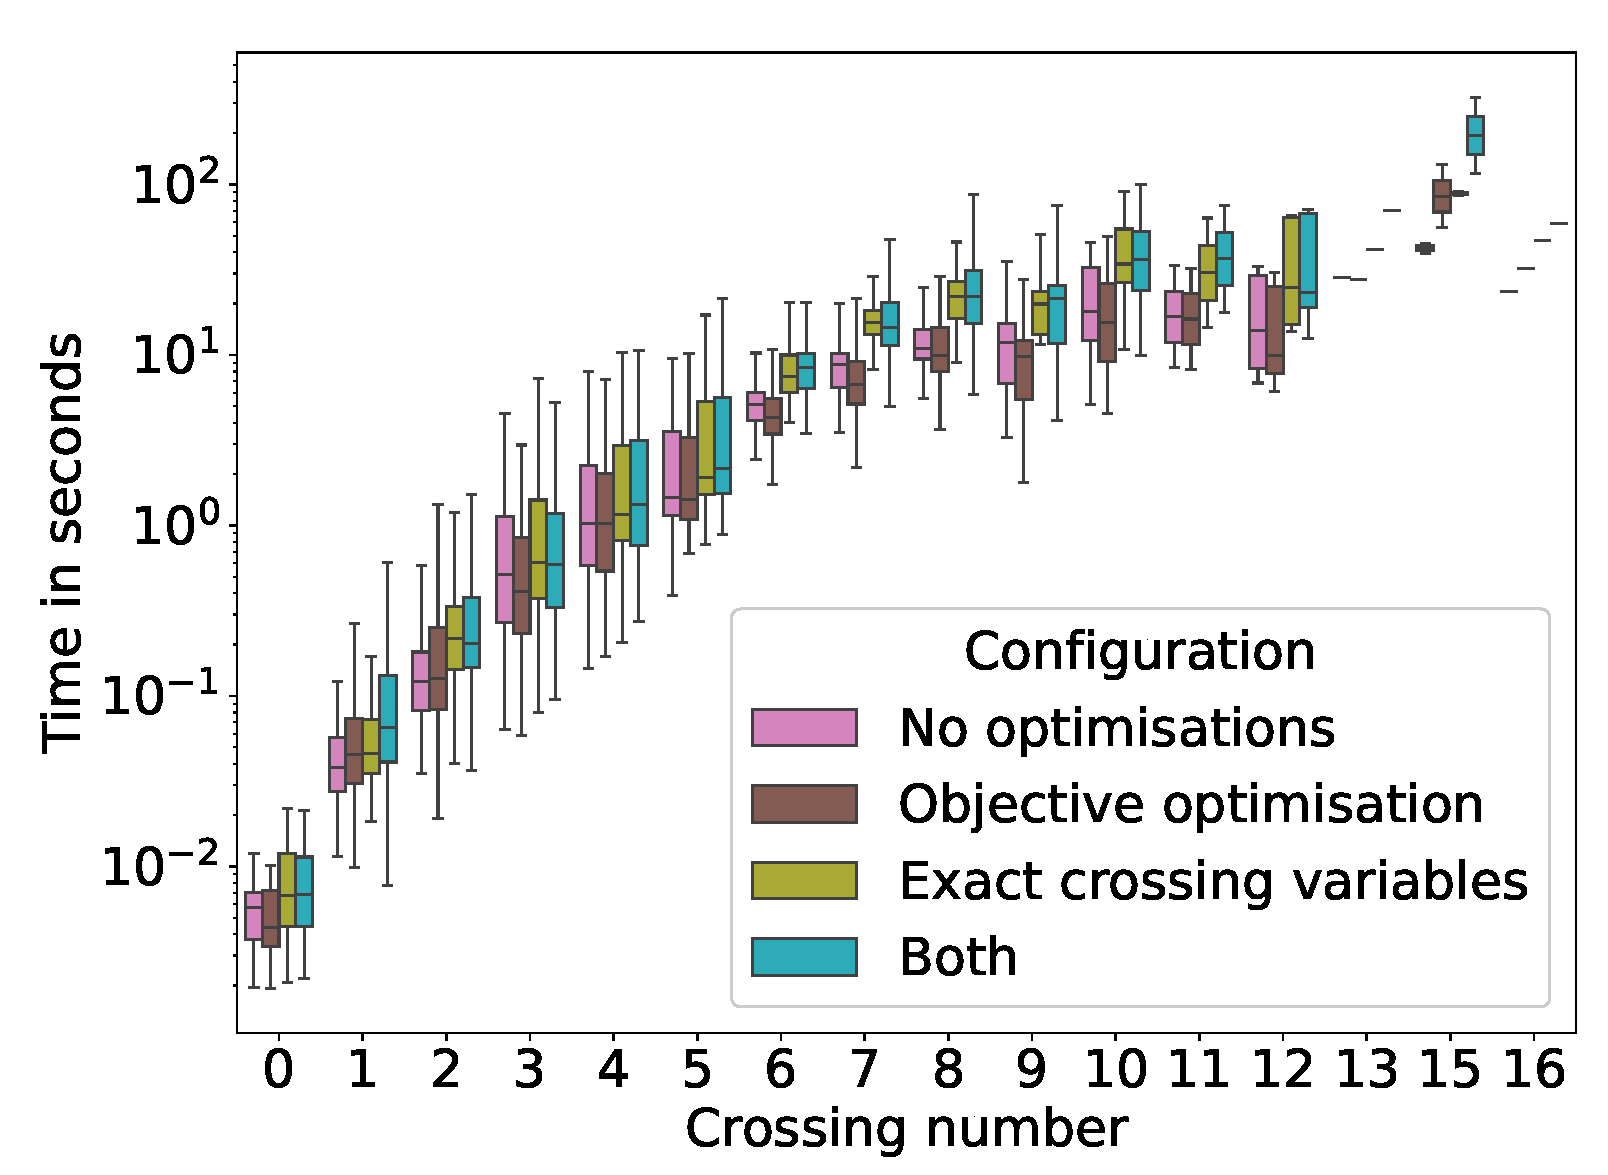
\includegraphics[width=0.47\textwidth]{experiments/ilp}
        \label{fig:optimisation:ilp}
    } \hfill
    \subfloat[SAT algorithm]{
        \includegraphics[width=0.47\textwidth]{experiments/sat}
        \label{fig:optimisation:sat}
    }
    \captionsetup{subrefformat=parens}
    \caption{Comparison of different configurations for ILP and SAT algorithms.}
    \label{fig:optimisation}
\end{figure}

The last experiment we considered is the comparison of optimisations we discussed for ILP and SAT methods in section~\ref{sec:optimisations}. For the ILP-based algorithm, we ran four configurations for each biconnected graph using none, one or both optimisations. For the SAT-based, we used two configurations with and without optimisation. The results are presented in figures~\ref{fig:optimisation:ilp} and~\ref{fig:optimisation:sat} respectively.

In the first plot, we can clearly see that adding additional constraints to enforce the exact value for each crossing variable degrades the performance. For SAT, however, this change does not influence this much. We can see a slight rise in execution time, but the difference is within the margin of error. Here, the difference might be caused by the algorithm writing down the required additional constraints, not the SAT solver.

The objective optimisation for the ILP, which includes an extra term in the objective function, makes small but still an improvement. As a result, we consider the algorithm that includes this optimisation to be the most efficient ILP-based algorithm. Thus, we have used this configuration for all other experiments. For the SAT method, we used a configuration that did not include optimisation.
